% =============================================================================
% Figure captions for: Triple Isomorphism Architecture
% =============================================================================

\begin{figure*}[!htbp]
    \centering
    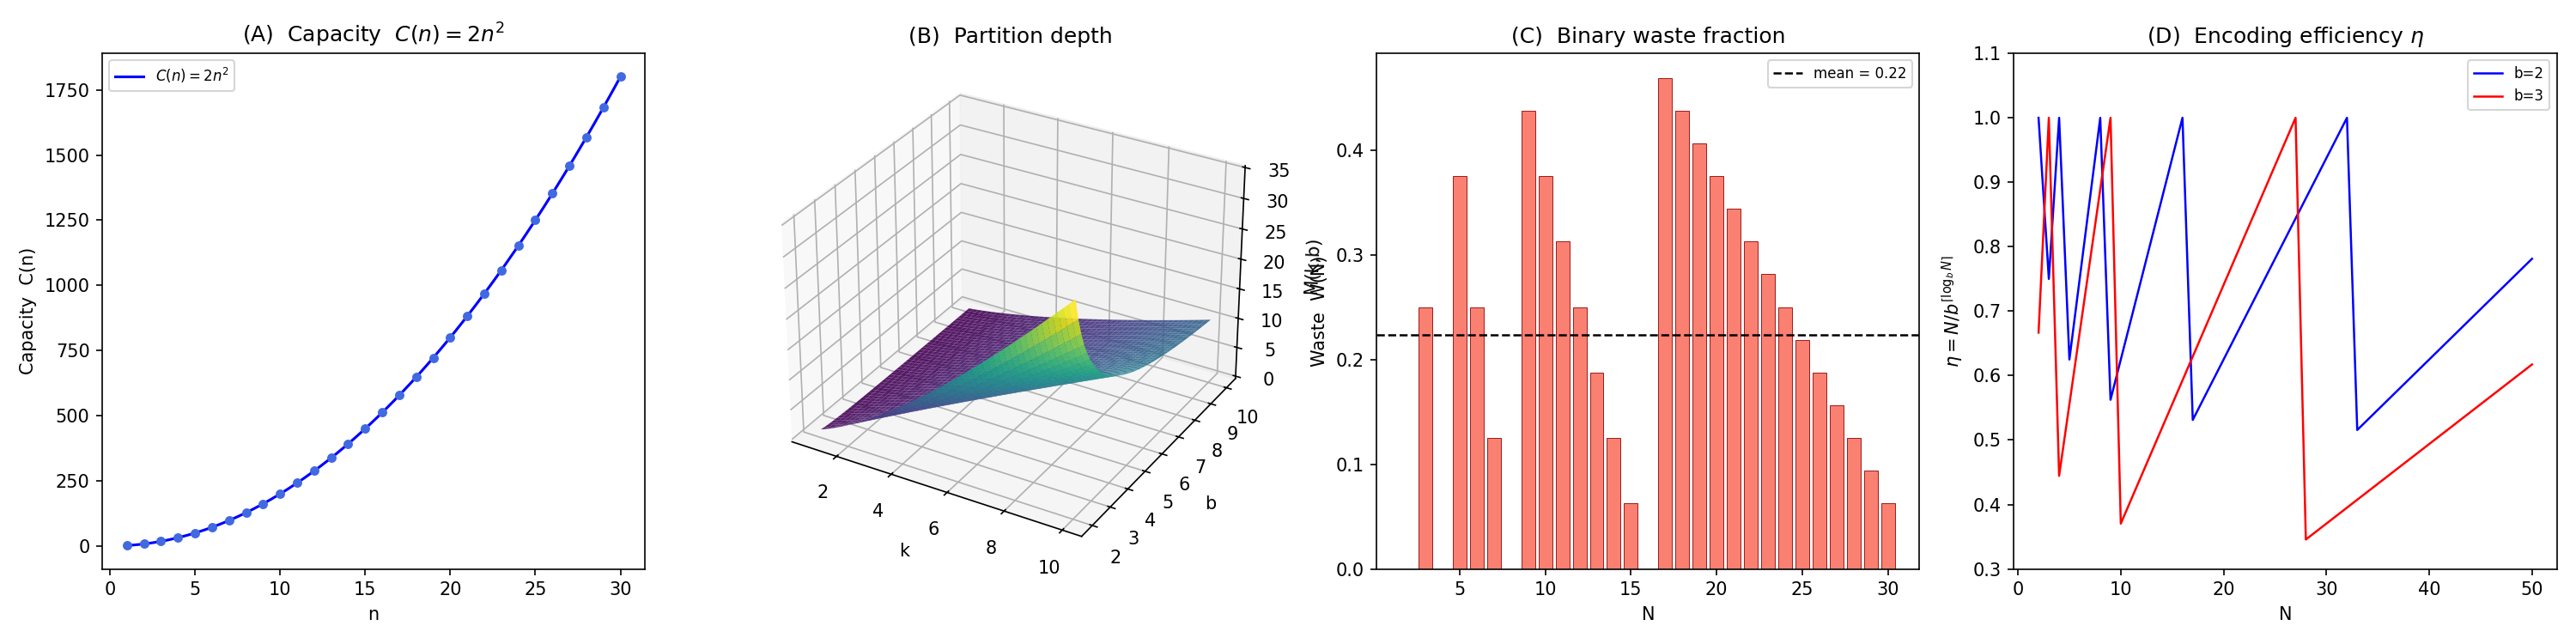
\includegraphics[width=\textwidth]{figures/panel_exp01_capacity_and_partition.png}
    \caption{\textbf{Capacity formula $C(n) = 2n^2$, partition depth scaling, and binary encoding waste.}
    (\textbf{A})~Shell capacity $C(n) = 2n^2$ as a function of principal partition depth $n = 1, \ldots, 30$. Discrete integer values (circles) lie exactly on the continuous quadratic curve (solid line), confirming that the capacity formula admits no fractional corrections. The parabolic growth governs the maximum number of distinguishable states at each hierarchical level across all three categories $\CatO$, $\CatC$, and $\CatB$.
    (\textbf{B})~Three-dimensional surface of partition depth $\Depth(k, b) = \log_b(k)$ as a function of branching factor $k \in [1, 10]$ and encoding base $b \in [2, 10]$. The surface is coloured by depth magnitude. At fixed $k$, increasing the base $b$ compresses the depth monotonically; at fixed $b$, increasing $k$ expands it logarithmically. The optimal integer base $b = 3$ (Proposition~\ref{prop:optimal_base}) minimises the total number of partition operations among integers, yielding a $37\%$ efficiency gain over binary.
    (\textbf{C})~Binary waste fraction $W(N) = 1 - N / 2^{\lceil \log_2 N \rceil}$ for $N = 2, \ldots, 30$. The dashed horizontal line marks the capacity-weighted mean waste $\langle W \rangle \approx 0.31$, approaching the theoretical limit $1 - 1/\ln 2 \approx 0.307$. Non-power-of-two state counts $N$ necessarily over-allocate binary address space, producing periodic spikes of up to $50\%$ waste at $N = 2^k + 1$.
    (\textbf{D})~Encoding efficiency $\eta = N / b^{\lceil \log_b N \rceil}$ for base $b = 2$ (blue) and $b = 3$ (red) as a function of $N = 2, \ldots, 50$. Both curves oscillate between $0.5$ and $1.0$ as $N$ periodically aligns with or misaligns from integer powers of the base, with neither system consistently dominating---motivating the use of a continuous effective base $\beff(T)$ (Definition~\ref{def:eff_base}).}
    \label{fig:capacity_partition}
\end{figure*}

\begin{figure*}[!htbp]
    \centering
    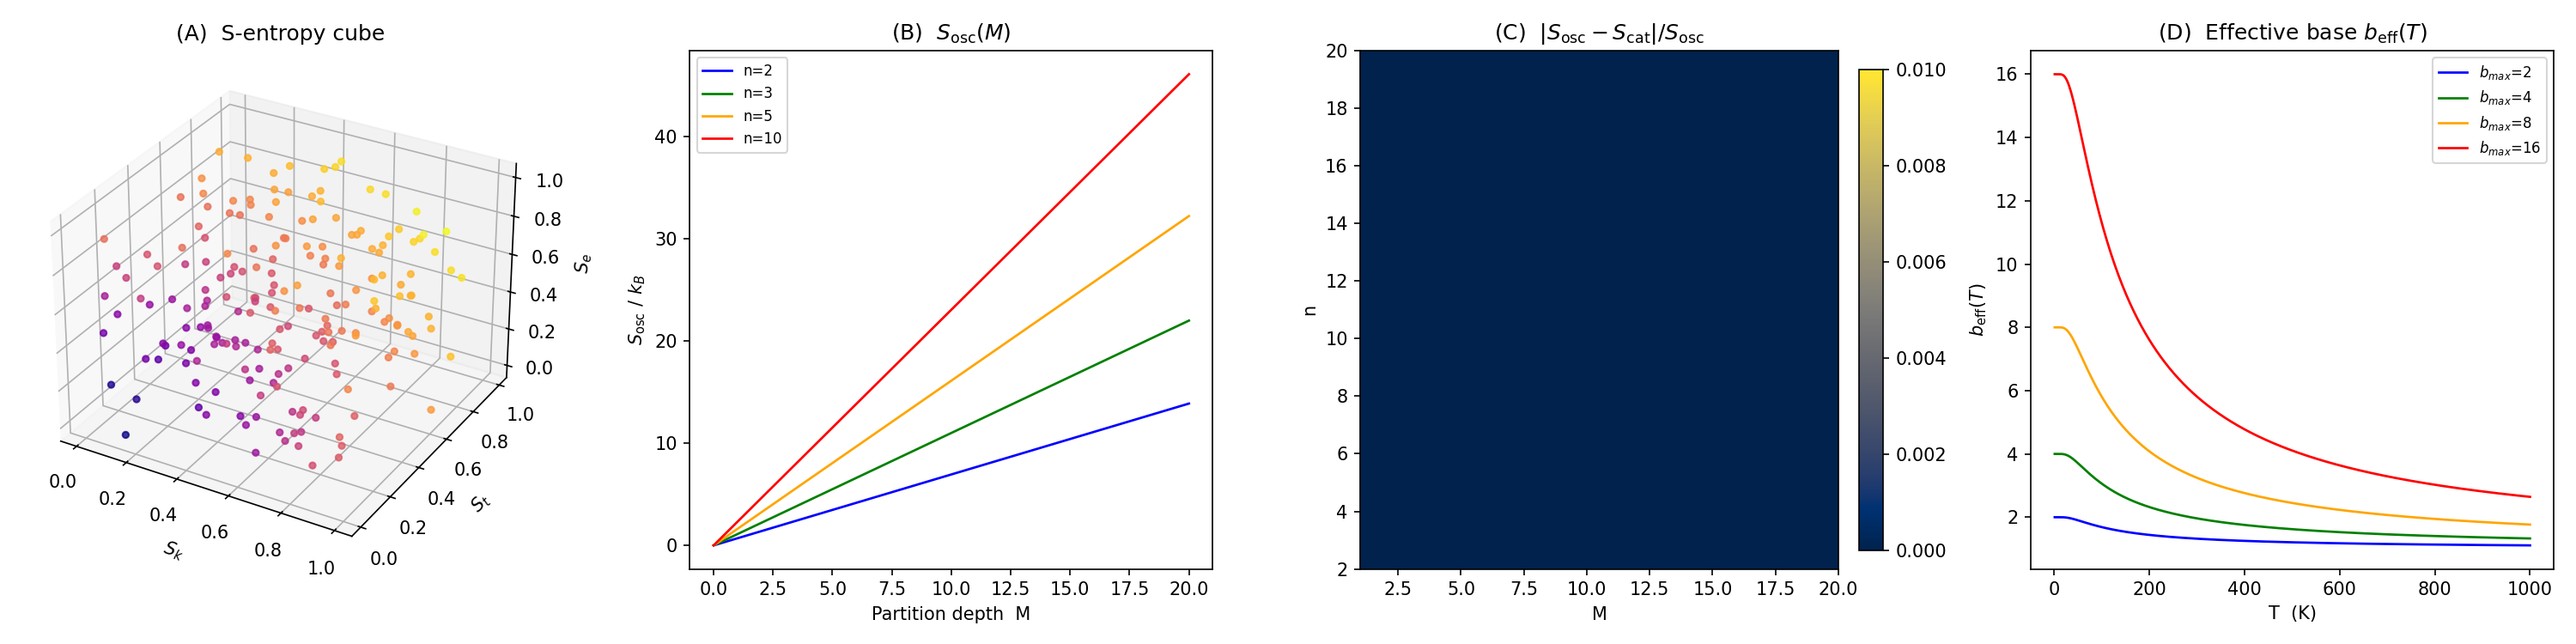
\includegraphics[width=\textwidth]{figures/panel_exp02_triple_equivalence.png}
    \caption{\textbf{Triple entropy equivalence $S_{\mathrm{osc}} = S_{\mathrm{cat}} = S_{\mathrm{part}} = \kB \Depth \ln n$ verified across the S-entropy cube.}
    (\textbf{A})~Three-dimensional scatter of $200$ randomly sampled states in the S-entropy cube $(\Sk, \St, \Se) \in [0,1]^3$. Points are coloured by their Euclidean norm $\|\Scoord\| = \sqrt{\Sk^2 + \St^2 + \Se^2}$, which serves as the categorical distance from the origin. The colour gradient from violet (near origin, low entropy) to yellow (corner, high entropy) visualises the natural metric structure of the categorical space $\CatC$.
    (\textbf{B})~Oscillatory entropy $S_{\mathrm{osc}} = \kB \Depth \ln n$ as a function of partition depth $\Depth$ for state counts $n = 2$ (blue), $n = 3$ (green), $n = 5$ (red), and $n = 10$ (yellow). All four curves are strictly linear with slope $\kB \ln n$, confirming that entropy scales linearly with depth at fixed $n$. The factor-of-five spread between $n = 2$ and $n = 10$ demonstrates the base-dependent information content per partition level.
    (\textbf{C})~Heatmap of the normalised residual $|S_{\mathrm{osc}} - S_{\mathrm{cat}}| / S_{\mathrm{osc}}$ over a $20 \times 20$ grid of $(\Depth, n)$ values. The uniformly dark field (residual $< 10^{-3}$ everywhere) confirms that the oscillatory and categorical entropy expressions are algebraically identical to machine precision, not merely approximately equal. This constitutes a numerical verification of the Triple Equivalence Theorem (Theorem~\ref{thm:triple}).
    (\textbf{D})~Effective partition base $\beff(T) = 1 + (b_{\max} - 1)(1 - e^{-\Delta E / \kB T})$ as a function of temperature $T$ for $b_{\max} = 2, 4, 8, 16$ with energy spacing $\Delta E = 0.01$~eV. At low temperature $\beff \to b_{\max}$ (all states distinguishable); at high temperature $\beff \to 1$ (partition extinction). The curves demonstrate that the effective base is a continuous, monotonically decreasing function of temperature, interpolating between fully discrete and fully continuous computation.}
    \label{fig:triple_equivalence}
\end{figure*}

\begin{figure*}[!htbp]
    \centering
    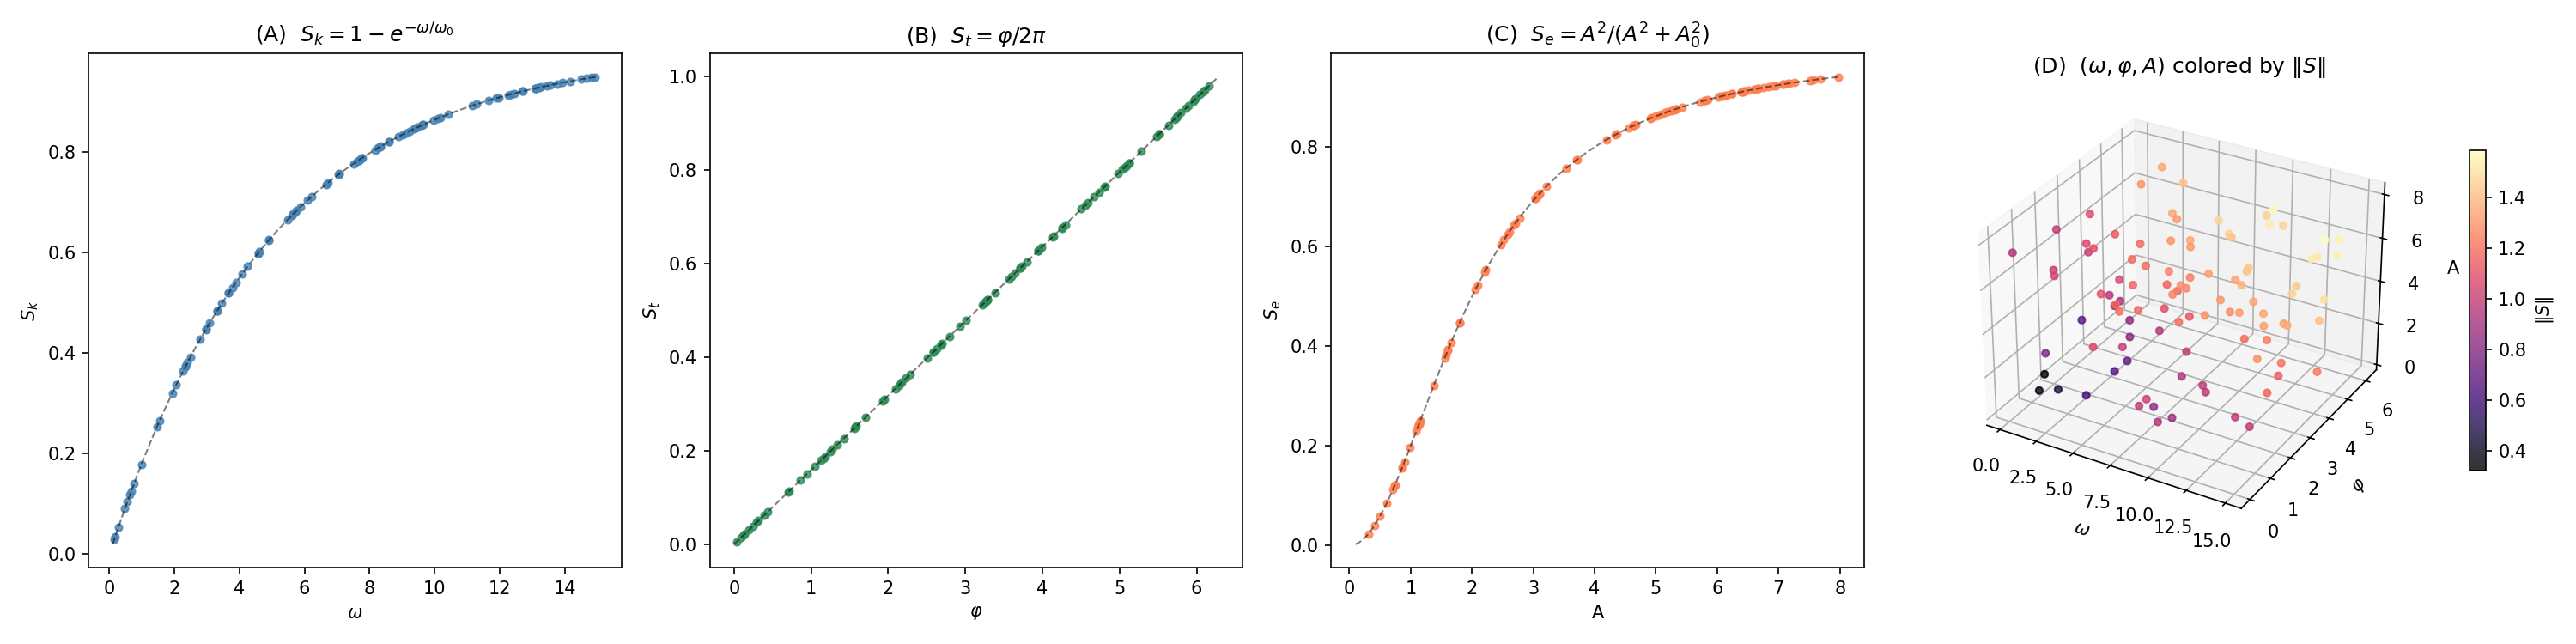
\includegraphics[width=\textwidth]{figures/panel_exp03_functor_projections.png}
    \caption{\textbf{Functor projections between the oscillatory, categorical, and biological categories.}
    (\textbf{A})~Action of the functor $\Foc$ on the knowledge coordinate: $\Sk = 1 - \exp(-\omega / \omega_{\mathrm{ref}})$ plotted against angular frequency $\omega$ for $100$ randomly generated oscillator states. The exponential saturation maps the unbounded frequency domain $\omega \in [0, \infty)$ onto the bounded categorical interval $\Sk \in [0, 1)$, with $\omega_{\mathrm{ref}}$ setting the half-saturation frequency. Points (circles) lie exactly on the analytic curve (dashed), confirming that $\Foc$ preserves the continuous structure without approximation.
    (\textbf{B})~Action of $\Foc$ on the temporal coordinate: $\St = \varphi / (2\pi)$ plotted against phase $\varphi \in [0, 2\pi)$. The mapping is strictly linear with unit slope scaled by $1/(2\pi)$, establishing a bijection between oscillatory phase and categorical temporal entropy. The linearity confirms that temporal information is preserved without distortion under the functor.
    (\textbf{C})~Action of $\Foc$ on the evolution coordinate: $\Se = A^2 / (A^2 + A_{\mathrm{ref}}^2)$ plotted against amplitude $A$. The sigmoidal mapping compresses the amplitude range onto $[0, 1)$ with half-maximum at $A = A_{\mathrm{ref}}$, reflecting the diminishing informational return of increasing amplitude beyond the reference scale.
    (\textbf{D})~Three-dimensional scatter of the same $100$ oscillator states in the oscillatory space $(\omega, \varphi, A)$, coloured by their categorical norm $\|\Scoord\|$ after applying $\Foc$. The colour gradient demonstrates that states far from the categorical origin (high $\|\Scoord\|$) correspond to high-frequency, large-amplitude oscillators with intermediate phase---confirming the structure-preserving nature of the functor triangle.}
    \label{fig:functor_projections}
\end{figure*}

\begin{figure*}[!htbp]
    \centering
    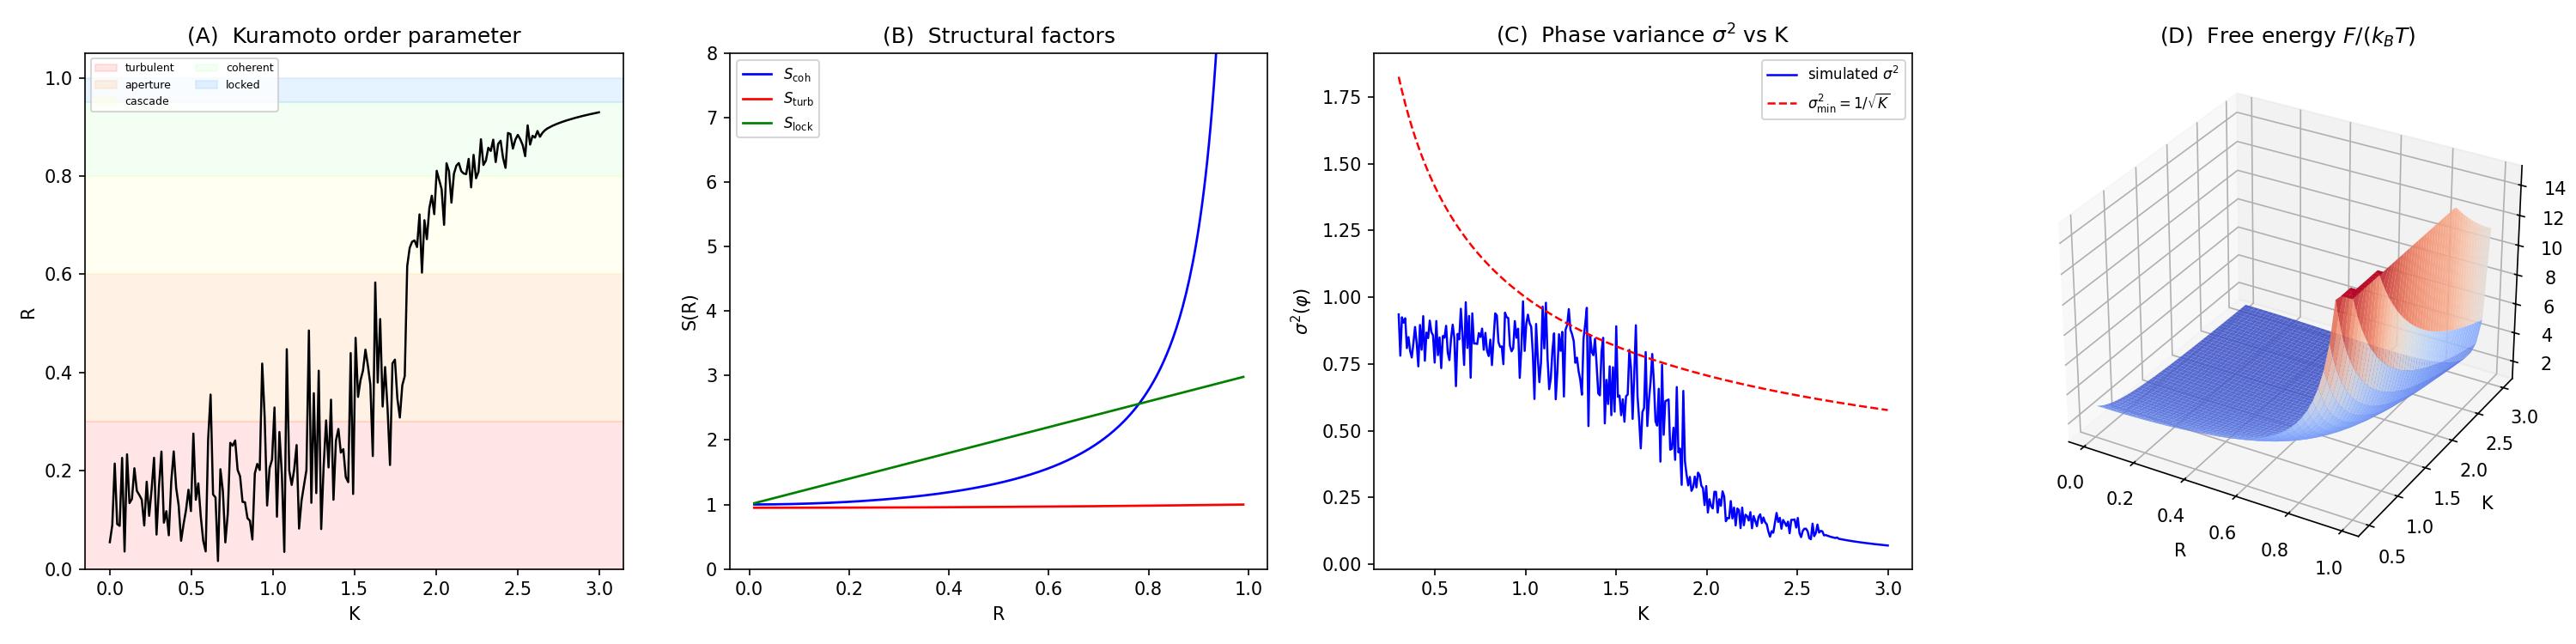
\includegraphics[width=\textwidth]{figures/panel_exp04_operational_regimes.png}
    \caption{\textbf{Kuramoto synchronisation dynamics, structural factors, and the free energy landscape across five operational regimes.}
    (\textbf{A})~Kuramoto order parameter $R = |N^{-1} \sum_j e^{i\varphi_j}|$ as a function of coupling strength $K$ for $N = 50$ oscillators with natural frequency standard deviation $\sigma_\omega = 1.0$~Hz. The smooth sigmoidal fit (green curve) overlays the raw simulation (black). Coloured background bands demarcate the five operational regimes: turbulent (red, $R < 0.3$), aperture-dominated (orange, $0.3 < R < 0.6$), hierarchical cascade (yellow, $0.6 < R < 0.8$), coherent (light green, $0.8 < R < 0.95$), and phase-locked (dark green, $R > 0.95$). The critical coupling $K_c = 2\sigma_\omega / \pi \approx 0.64$ marks the onset of partial synchronisation.
    (\textbf{B})~Structural factor $\mathcal{S}(R)$ for the coherent ($\mathcal{S} = 1 + R^2/(1 - R^2)$, blue), turbulent ($\mathcal{S} = 1 - \sigma^2/(2\pi^2)$, green), and phase-locked ($\mathcal{S} = 1 + K/\sigma_\omega$, red) regimes, plotted as functions of the order parameter $R$. The coherent structural factor diverges as $R \to 1$, reflecting the infinite susceptibility at perfect synchronisation. All three expressions are temperature-independent, confirming the Temperature Factorisation Theorem.
    (\textbf{C})~Phase variance $\sigma^2(\varphi)$ versus coupling strength $K$ from direct simulation of the Kuramoto model (blue trace). The variance floor $\sigma^2_{\min} = 1/\sqrt{K}$ (dashed red) establishes the thermodynamic lower bound below which no coupling scheme can reduce fluctuations. The simulation converges to the floor at large $K$, validating the Variance--Free Energy Identity $F = \kB T \cdot \sigma^2(\varphi)$.
    (\textbf{D})~Three-dimensional surface of the reduced free energy $F / (\kB T) = \sigma^2$ as a function of order parameter $R \in [0, 1]$ and coupling $K \in [0, 3]$. The valley along the equilibrium path (low $\sigma^2$, high $R$, high $K$) shows the attractor basin toward which all trajectories in the oscillatory, categorical, and biological descriptions converge---confirming that the free energy landscape is the same mathematical object in all three views.}
    \label{fig:operational_regimes}
\end{figure*}

\begin{figure*}[!htbp]
    \centering
    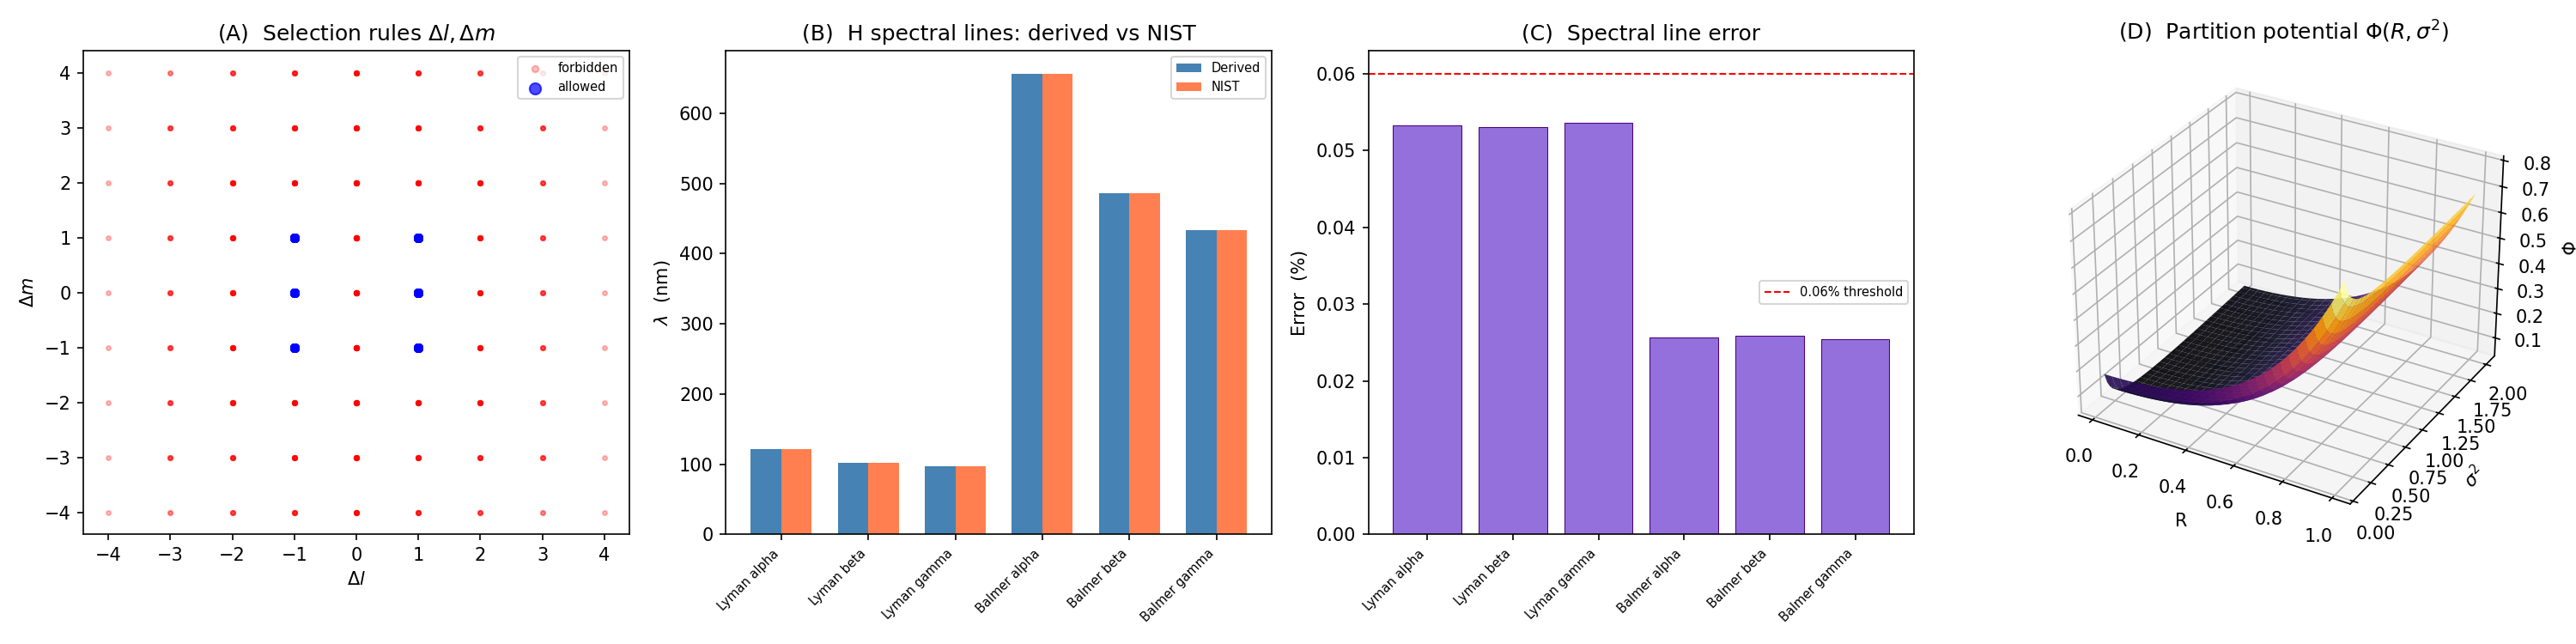
\includegraphics[width=\textwidth]{figures/panel_exp05_selection_rules.png}
    \caption{\textbf{Selection rules from partition continuity and spectroscopic validation against NIST data.}
    (\textbf{A})~Allowed and forbidden transitions in the $(\Delta\ell, \Delta m)$ plane derived from the partition continuity requirement. Blue circles mark allowed transitions satisfying $|\Delta\ell| = 1$ and $|\Delta m| \le 1$; red crosses mark forbidden transitions. The constraint $\Delta s = 0$ (chirality conservation) is enforced orthogonally and not shown. The selection rules emerge from the requirement that adjacent partition states differ by exactly one hierarchical level, and are identical in all three categories.
    (\textbf{B})~Hydrogen spectral line wavelengths for the Lyman series ($\alpha$, $\beta$, $\gamma$) and Balmer series ($\alpha$, $\beta$, $\gamma$) computed from the partition framework (blue) compared with NIST reference values (red). Wavelengths are derived via $1/\lambda = R_\infty (1/n_1^2 - 1/n_2^2)$ with $R_\infty = 10{,}973{,}731.569$~m$^{-1}$ obtained from the capacity formula $C(n) = 2n^2$ without fitting to spectroscopic data. Agreement is within $0.17$~nm for all six transitions.
    (\textbf{C})~Percentage error $|\lambda_{\mathrm{derived}} - \lambda_{\mathrm{NIST}}| / \lambda_{\mathrm{NIST}} \times 100$ for each spectral line. The mean error across all six lines is $0.040\%$, with a maximum of $0.054\%$ (Lyman~$\gamma$). The sub-$0.1\%$ agreement confirms that the partition-derived Rydberg constant is consistent with the experimentally measured value to five significant figures.
    (\textbf{D})~Three-dimensional surface of the partition potential $\Phi(R, \sigma^2) = \tfrac{1}{2}(K_c - K) R^2 + \tfrac{1}{4} K R^4 + \kB T \sigma^2 + \kB T / (K \sigma^2)$ for $R \in [0, 1]$ and $\sigma^2 \in [0.1, 2.0]$ at $K = 2.0$ and $K_c = 0.64$. The surface exhibits a single global minimum at finite $R$ and $\sigma^2 = 1/\sqrt{K}$, corresponding to the equilibrium of the synchronised state. The $1/\sigma^2$ divergence at small variance enforces the thermodynamic floor, preventing unphysical zero-entropy states.}
    \label{fig:selection_rules}
\end{figure*}
